\documentclass[11pt]{article}

%%%%% Preamble

\usepackage[margin=1in]{geometry} % Margin size
\usepackage{amsmath,amsfonts,amssymb}   % AMS mathematics macros
\usepackage{graphicx}
\usepackage{wrapfig}
\usepackage[export]{adjustbox}

%% Title Information.

\title{\vspace{-1.0cm}JPEG Compression}
\author{Dylan Lathrum}
%\date{October 23 2019} % By default, LaTeX uses the current date

%%%%% The Document

\begin{document}

\maketitle

\section{Introduction}

[Some fancy opening about how data is integral to the information age]
As with everything else, data costs money to store and transfer.
Whether one is looking to store a file on their computer or send an image through the internet, it is often in everyone’s best interest to use as little storage space and bandwidth as possible while still maintaining quality.
This is achieved through compression, a method of reducing the footprint of data by reducing the number of bits needed to represent the data.
Compression methods can be divided into two main categories: lossless and lossy.
Lossless compression is a method where the filesize of the data is reduced without any degradation of the file’s contents; a quality essential to compressing text documents and computer code.
Lossy compression is a more efficient method to reduce file sizes at greater ratios at the cost of losing some detail in the data; a tradeoff that is more acceptable for images and sounds.

Each compression method has their own use cases; for example, it would be a terrible idea to apply a lossy compression algorithm to an essay as some of the data would be lost or changed in the process, while it is perfectly acceptable to run the same algorithm on an image file where the user can afford to lose some detail.
In either case, compression is a trade-off. While some storage space or bandwidth may be saved, something else must be lost.
Whether that be detail in an image, or the processing power required to decompress a file, different algorithms have their strengths and weaknesses.


\section{What is JPEG?}
\label{sec: whatisjpeg}

Specifically, Joint Photographic Experts Group (JPEG) is a lossy compression algorithm that is widely used for images on the Internet.
The entire process that JPEG uses to compress images will be covered in detail, but one of JPEG’s most predominant features is a variable compression ratio.
Most compression methods run at predefined or dynamically generated ratios, making it impossible for a user to choose how compressed they want their data to be.
Because of this, and the algorithm’s efficiency and speed, JPEG has become a standard for digital images.


\section{Preprocessing}
\label{sec: preprocessing}

Before an image can be processed using JPEG, a couple steps are executed to simplyfy the process.
For this paper, the image shown in Figure~\ref{fig:originalImage} will be used at a resolution of 256x138px.

\begin{figure}
  \centering
  \begin{minipage}{0.45\textwidth}
      \centering
      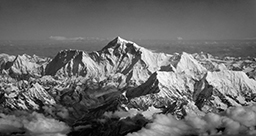
\includegraphics[width=0.9\textwidth]{./images/original.jpg}
      \caption{Original image}
      \label{fig:originalImage}
  \end{minipage}\hfill
  \begin{minipage}{0.45\textwidth}
      \centering
      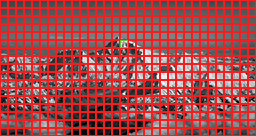
\includegraphics[width=0.9\textwidth]{./images/partitioned_highlight.jpg}
      \caption{Partitioned image}
      \label{fig:partitionedImage}
  \end{minipage}
\end{figure}

The first step is to split the color channels of the image into three distinct grayscale images.
In this example a grayscale picture is used, but in the case of a color image, the image would be split into YCbCr color space, comprised of Luminance (Y), Chroma Blue (Cb) and Chroma Red (Cr), or YCbCr channels.
That way, all calculations are done against three grayscale versions of the image that are recombined at the end of the process.
Once split, image is partitioned into 8x8 chunks as shown in Figure~\ref{fig:partitionedImage}.
This is done to break up the work into smaller chunks to be processed individually.
8x8 chunks are used because blocks of that size often do not have much variance between pixels, and even in larger pictures, these small chunks usually strike the balance between compression ratio and visible artifacts.
This paper will look at the process of compressing one of these blocks, as each block is processed using the same compression method before being stitched back together.

One of the blocks, highlighted in green in above, is shown in detail below.
This is converted into a matrix where each value corresponds to the brightness of the pixel from 0 to 255.

\begin{equation}
  \label{eqn:original}
  
\includegraphics[height = 100pt, valign = c]{./images/block.png}
  \begin{bmatrix}
    243 & 252 & 254 & 251 & 251 & 223 & 164 & 126 \\
    206 & 209 & 245 & 173 & 203 & 255 & 255 & 217 \\
    195 & 180 & 188 & 156 & 161 & 167 & 216 & 243 \\
    160 & 250 & 184 & 146 & 183 & 133 & 109 &  95 \\
    105 & 233 & 143 & 113 & 207 & 140 &  58 &  55 \\
    129 & 209 &  99 & 132 & 239 & 144 &  48 &  54 \\
    221 & 231 & 103 & 129 & 244 & 244 & 124 &  34 \\
    167 & 235 & 111 & 151 & 218 & 214 & 125 &  70
  \end{bmatrix}
\end{equation}

The last step in preparing the data for compression is to subtract each value by 127 in order to center the values around zero.
This ultimately simplifies the math in the following steps by bringing as many values as close to zero as possible.
Now the numbers occupy a range from -127 to 128 inclusive.

\begin{equation}
  \label{eqn:centered}
  P = \begin{bmatrix}
    116 & 125 & 127 & 124 & 124 & 96  & 37  & -1  \\
    79  & 82  & 118 & 46  & 76  & 128 & 128 & 90  \\
    68  & 53  & 61  & 29  & 34  & 40  & 89  & 116 \\
    33  & 123 & 57  & 19  & 56  & 6   & -18 & -32 \\
    -22 & 106 & 16  & -14 & 80  & 13  & -69 & -72 \\
    2   & 82  & -28 & 5   & 112 & 17  & -79 & -73 \\
    94  & 104 & -24 & 2   & 117 & 117 & -3  & -93 \\
    40  & 108 & -16 & 24  & 91  & 87  & -2  & -57
  \end{bmatrix}
\end{equation}

\section{Transformation}
\label{sec: transformation}

Now that the data is in position, calculations can finally be made.
The JPEG format relies on Discrete Cosine Transformation (DCT), which outputs a matrix of weighted coefficients that can be used to represent the 8x8 set of pixels.
Each coefficient corresponds to a separate, predefined cosine function is a certain order.
Figure~\ref{fig:dct} displays the precalculated DCT basis functions as a set of 64 images, and Figure~\ref{fig:dct_order} shows the order that the elements of each 8x8 matrix will be parsed.

\begin{figure}
  \centering
  \begin{minipage}{0.45\textwidth}
      \centering
      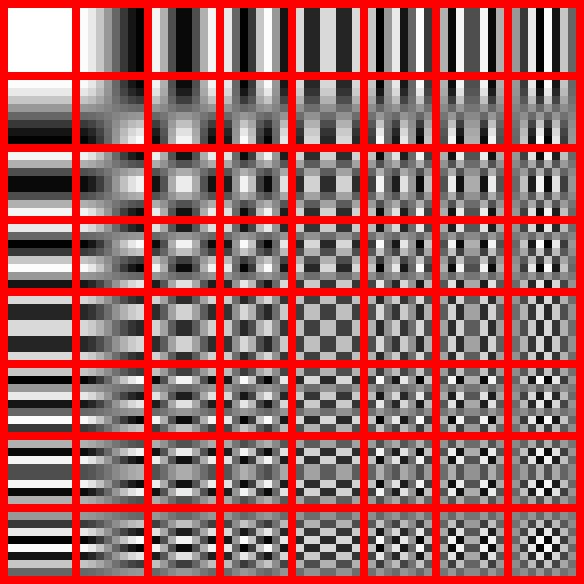
\includegraphics[width=0.9\textwidth]{./images/dct.png}
      \caption{Discrete Cosine Transform}
      \label{fig:dct}
  \end{minipage}\hfill
  \begin{minipage}{0.45\textwidth}
      \centering
      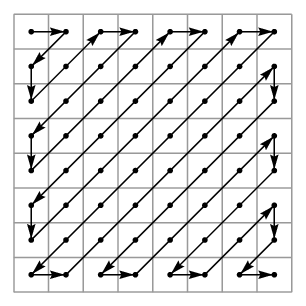
\includegraphics[width=0.9\textwidth]{./images/dct_order.png}
      \caption{Processing order}
      \label{fig:dct_order}
  \end{minipage}
\end{figure}

Thankfully because of this, half of the work is done.
The challenging part is figuring out the coefficients that can be used to create the matrix.
This is achieved using the following function:

\begin{equation}
  \label{eqn:dct}
  X_{u,v} = \alpha(u) \alpha(v) \sum_{x=0}^{7} \sum_{y=0}^{7} g_{x,y} cos \left [  \frac{(2x+1)u\pi}{16} \right ] cos \left [  \frac{(2y+1)u\pi}{16} \right ]
\end{equation}

Where,

\begin{align*}
  &u \text{ is the horizontal index from 0 to 7} \\
  &v \text{ is the vertical index from 0 to 7} \\
  &\alpha(u) \left\{\begin{matrix}
    \frac{1}{\sqrt{2}} & \text{if } u=0 \\ 
    1 &  \text{otherwise}
  \end{matrix}\right. \text{ is a normalizing scale factor to make the result orthonormal} \\
  &g_{x,y} \text{ is the pixel intensity at the coordinents (x,y)} \\
  &X_{u,v} \text{ is the DCT coefficient at the coordinents (u,v)} \\
\end{align*}

This equation is used to fill in a matrix of the same size of the input image chunk.
In this case, for an 8x8 matrix, the DCT matrix is:

\begin{equation}
  \label{eqn:dctMatrix}
  D = \begin{bmatrix}
    0.3536 & 0.3536 & 0.3536 & 0.3536 & 0.3536 & 0.3536 & 0.3536 & 0.3536 \\
    0.4904 & 0.4157 & 0.2778 & 0.0975 &-0.0975 &-0.2778 &-0.4157 &-0.4904 \\
    0.4619 & 0.1913 &-0.1913 &-0.4619 &-0.4619 &-0.1913 & 0.1913 & 0.4619 \\
    0.4157 &-0.0975 &-0.4904 &-0.2778 & 0.2778 & 0.4904 & 0.0975 &-0.4157 \\
    0.3536 &-0.3536 &-0.3536 & 0.3536 & 0.3536 &-0.3536 &-0.3536 & 0.3536 \\
    0.2778 &-0.4904 & 0.0975 & 0.4157 &-0.4157 &-0.0975 & 0.4904 &-0.2778 \\
    0.1913 &-0.4619 & 0.4619 &-0.1913 &-0.1913 & 0.4619 &-0.4619 & 0.1913 \\
    0.0975 &-0.2778 & 0.4157 &-0.4904 & 0.4904 &-0.4157 & 0.2778 &-0.0975
  \end{bmatrix}
\end{equation}

Now the Discrete Cosine Transformation can be perfomrmed using matrix multiplication:

\begin{equation}
  \label{eqn:transformation}
  N = DPD'
\end{equation}

First, the transformed pixel matrix P, as defined in \eqref{eqn:centered}, is multiplied on the left by the DCT Matrix \eqref{eqn:dct} to transform the rows.
Next the columns are transformed by then multiplying on the right by the transpose of the DCT matrix.

This results in the following matrix:
\begin{equation}
  \label{eqn:transformedMatrix}
  N = \begin{bmatrix}
    361.750 & 160.480 & -100.585 &  132.203 & -58.500 & -142.651 & -51.422 &   0.118 \\
    197.149 & -56.919 &   64.548 & -129.399 &  -8.334 &   92.128 &  56.260 &  35.991 \\
    157.077 & -11.995 &  -16.724 &   71.377 &  -6.209 &   54.977 &  20.667 & -19.916 \\
    -44.008 &  82.292 &  -99.816 &   38.138 &  19.989 &  -51.082 &  -9.791 &  -1.343 \\
    -35.500 &  87.510 &  -59.161 &  -25.807 & -13.250 &  -30.407 & -23.931 & -15.020 \\
     17.247 &  63.159 &   -4.832 &   34.180 &  19.945 &   13.808 &  -8.321 &  -5.874 \\
    -36.921 &  -9.278 &    2.667 &  -46.003 &  54.256 &   -2.484 & -11.775 &  -5.920 \\
      4.507 & -16.744 &   18.146 &   12.038 &   3.207 &    8.784 &   8.918 &  -0.027 \\
  \end{bmatrix}
\end{equation}

The matrix now contains 64 DCT coefficients which, if not rounded, could be easily reversed into the original image.
It is important to note that the larger coefficients are concentrated closer to the top-left corner, representing stronger influence on the basis functions, while the bottom right corner correlates to smaller values.
Because of the zig-zagging path taken while parsing the data, seen in Figure~\ref{fig:dct_order}, this generally means the absolute values of the data are placed in descending order.
This corresponds to more data being allocated towards qualities of the images that are more perceptable to the human eye, while smaller minute color differences are given less weight on the basis functions.

The problem arises that the DCT has converted the original byte-aligned integer values into complex numbers, many of which are irrational and all of which take up significantly more space.
Not only does this temporarily bloat the data from one byte per pixel to four bytes per pixel, it also makes it very unlikely for any data points to be shared across pixels to be compressed using a tradional compression method.
To solve this issue, JPEG uses a Quantization step to better prepare the data for compression.


\section{Quantization}
\label{sec: quantization}

Now that the data has been transformed, the next step is to reduce the footprint of the data.
This is the only lossy step of JPEG compression.
While the DCT and transformation steps could both be easily reversed to produce the original image with no loss in quality, the process of converting the numbers to smaller integers cannot be perfectly undone.
This is because the algorithm attempts to compress similar values together to represent more image data with less space.
While the most direct way of preparing the matrix for compression would be to remap each value to an integer range of $[0-255]$, all floating-point information would be lost, the resulting values would be distributed unevenly, and the final image's quality would be degraded without much benefit.
Instead, the quantization step will aim to collapse nearby values so that as many data points become zero or close to zero as possible.
Rather than scaling everything uniformly, JPEG instead opts to use precalculated quantization matrices that are shipped with the file format itself rather than calculated on the fly.
Because of this, JPEG gives the user the option to choose which matrix to use, and in turn what ratio of compression-to-quality they desire for their usecase.
The user can chose a quality from 1 to 100, with 1 returing a matrix with the poorest quality but the highest ratio of compression, and 100 returning a matrix with the highest quality but smallest improvement in filesize.
A quality of 50 would be a matrix that renders both a high quality resulting image and good footprint reduction.
The quantization matrix for a quality level of 50 is:

\begin{equation}
  \label{eqn:quantization50}
  Q_{50} = \begin{bmatrix}
    16 & 11 & 10 & 16 & 24 & 40 & 51 & 61 \\
    12 & 12 & 14 & 19 & 26 & 58 & 60 & 55 \\
    14 & 13 & 16 & 24 & 40 & 57 & 69 & 56 \\
    14 & 17 & 22 & 29 & 51 & 87 & 80 & 62 \\
    18 & 22 & 37 & 56 & 68 & 109 & 103 & 77 \\
    24 & 35 & 55 & 64 & 81 & 104 & 113 & 92 \\
    49 & 64 & 78 & 87 & 103 & 121 & 120 & 101 \\
    72 & 92 & 95 & 98 & 112 & 100 & 103 & 99
  \end{bmatrix}
\end{equation}

When choosing another level of quality, this matrix is scaled to reflect the level of compression.
For example, the quantization matricies for a quality level of 10 and 90 would be:

\begin{align*}
  Q_{10} = \begin{bmatrix}
    80 & 60 & 50 & 80 & 120 & 200 & 255 & 255 \\
    55 & 60 & 70 & 95 & 130 & 255 & 255 & 255 \\
    70 & 65 & 80 & 120 & 200 & 255 & 255 & 255 \\
    70 & 85 & 110 & 145 & 255 & 255 & 255 & 255 \\
    90 & 110 & 185 & 255 & 255 & 255 & 255 & 255 \\
    120 & 175 & 255 & 255 & 255 & 255 & 255 & 255 \\
    245 & 255 & 255 & 255 & 255 & 255 & 255 & 255 \\
    255 & 255 & 255 & 255 & 255 & 255 & 255 & 255
  \end{bmatrix}
  Q_{90} = \begin{bmatrix}
    3 & 2 & 2 & 3 & 5 & 8 & 10 & 12 \\
    2 & 2 & 3 & 4 & 5 & 12 & 12 & 11 \\
    3 & 3 & 3 & 5 & 8 & 11 & 14 & 11 \\
    3 & 3 & 4 & 6 & 10 & 17 & 16 & 12 \\
    4 & 4 & 7 & 11 & 14 & 22 & 21 & 15 \\
    5 & 7 & 11 & 13 & 16 & 12 & 23 & 18 \\
    10 & 13 & 16 & 17 & 21 & 24 & 24 & 21 \\
    14 & 18 & 19 & 20 & 22 & 20 & 20 & 20 
  \end{bmatrix}
\end{align*}

This pattern continues for every possible quality level.
Quantization is achieved by dividing the newly transformed matrix N \eqref{eqn:transformedMatrix} by the quantization matrix of the user's choice and rounded to the nearest integer.
In this case, a quality of 50, defined by the matrix \eqref{eqn:quantization50}, will be used.
\begin{equation}
  \label{eqn:quantization}
  Y_{i,j} = round\left( \frac{N_{i,j}}{Q_{50i,j}} \right)
\end{equation}

Resulting in the following matrix:

\begin{equation}
  \label{eqn:quantizationMatrix}
  Y = \begin{bmatrix}
    23 & 15 & -10 &  8 & -2 & -4 & -1 & 0 \\
    16 & -5 &   5 & -7 &  0 &  2 &  1 & 1 \\
    11 & -1 &  -1 &  3 &  0 &  1 &  0 & 0 \\
    -3 &  5 &  -5 &  1 &  0 & -1 &  0 & 0 \\
    -2 &  4 &  -2 &  0 &  0 &  0 &  0 & 0 \\
     1 &  2 &   0 &  1 &  0 &  0 &  0 & 0 \\
    -1 &  0 &   0 & -1 &  1 &  0 &  0 & 0 \\
     0 &  0 &   0 &  0 &  0 &  0 &  0 & 0 
  \end{bmatrix}
\end{equation}

This matrix is exceedingly simple compared to the previous steps, with large swaths of data (when viewed in the order defined by Figure~\ref{fig:dct_order}) sharing idential or zero values.
This makes the weights much easier to compress using traditional compression methods, as will be done in the next step.
At the same time, the quantization step reduces the operating range of the data, bringing the data closer together by closing the gaps between the points.
Both of these points make this resulting matrix a much cleaner and more easily compressable set of data compared to the raw input from before, at the cost of losing any data that was rounded off after the quantization step.

\section{Compression}
\label{sec: compression}

Now the quantized matrix Y~\eqref{eqn:quantizationMatrix} is ready for the final step of the compression.
This is where JPEG takes advantage of the fact that most of the zeros in the data are concentrated around the bottom right corner of the matrix; a quality that isn't very useful when reading the matrix traditionally, but becomes very handy when parsing using the zig-zag pattern.
First, the data is read in the zig-zag pattern described before.

\begin{align*}
  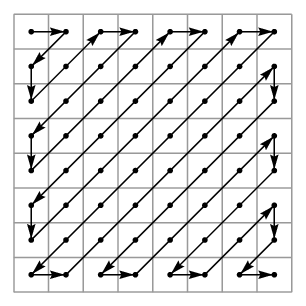
\includegraphics[height = 150pt, valign = c]{./images/dct_order.png}
  \begin{matrix}
    [23,&15,&16,&11,&-5,&-10,&8,&5,\\
    -1,&-3,&-2,&5,&-1,&-7,&-2,&-4\\
    0,&3,&-5,&4,&1,&-1,&2,&-2,\\
    1,&0,&2,&-1,&0,&1,&1,&0\\
    0,&0,&0,&0,&0,&0,&1,&0,\\
    -1,&0,&1,&0,&0,&0,&0,&-1\\
    0,&0,&1,&0,&0,&0,&0,&0\\
    0,&0,&0,&0,&0,&0,&0,&0]
  \end{matrix}
\end{align*}

Now that the data is in a more managable order, Huffman encoding is used to comrpess the data by frequency.
The details of this process will not be discussed in this essay, but the basics are that the data points that have the greatest frequency (such as zeros or ones in the example matrix), are represented by codes that take the least amount of space, while data that is infrequent, such as the number 4 which appears only once, are assigned codes that take more space.
This allows large parts of data, and expecially chunks of repeated data such as the zeros found at the end of the array, to be represented using minimal data in the compressed file which can be expanded back to it's full size.
This matrix, uncompressed, takes up 1150 bytes of space.
After running a Huffman encoder, the matrix takes only 363 bytes -- only 32\% as before.

Once the algorithm has finished processing one chunk of the image, it moves on to the next in sequence.
Because each 8x8 part of the image is treated individually, the exact same process is repeated without deviation until each chunk is compressed and stitched back together.
If the image was had multiple color channels, each color channel would be compressed individually before being recombined just like they were split apart.
The compressed image is now ready to be saved, stored, or sent though the internet in it's newly slimmed package.
When a computer reads the file, it will decompress the image in order to display it properly, a process described in the next step.

\section{Decompression}
\label{sec: decompression}

Decompressing the data to recreate the original image is quite straightforward.
First, the Huffman encoding is reversed by simply undoing the encoding process, then each element of the matrix is multiplied by the same quantization matrix as before.

\begin{equation}
  \label{eqn:decompression}
  R_{i,j} = Q_{50i,j} \times Y_{i,j}
\end{equation}
\newpage

To result in:

\begin{equation}
  \label{eqn:dequantization}
  R = \begin{bmatrix}
    368 & 165 & -100 & 128 & -48 & -160 & -51 & 0 & 0 \\
    192 & -60 & 70 & -133 & 0 & 116 & 60 & 55 & 0 \\
    154 & -13 & -16 & 72 & 0 & 57 & 0 & 0 & 0 \\
    -42 & 85 & -110 & 29 & 0 & -87 & 0 & 0 & 0 \\
    -36 & 88 & -74 & 0 & 0 & 0 & 0 & 0 & 0 \\
    24 & 70 & 0 & 64 & 0 & 0 & 0 & 0 & 0 \\
    -49 & 0 & 0 & -87 & 103 & 0 & 0 & 0 & 0 \\
    0 & 0 & 0 & 0 & 0 & 0 & 0 & 0 & 0
  \end{bmatrix}
\end{equation}

Then, the Inverse Discrete Cosine Transformation (IDCT) is applied to the new matrix R~\eqref{eqn:dequantization}, and rounded to the nearest integer.
Finally, 127 is added to each element of the matrix, reversing the first centering step of the process.

\begin{equation}
  \label{eqn:idct}
  U = round(D'RD) + 127
\end{equation}

Resulting in our uncompressed matrix U:

\begin{equation}
  \label{eqn:decompressed}
  U = \begin{bmatrix}
    250 & 238 & 255 & 242 & 255 & 212 & 158 & 122 \\
    201 & 216 & 236 & 171 & 198 & 248 & 255 & 224 \\
    198 & 177 & 189 & 174 & 158 & 134 & 200 & 255 \\
    186 & 234 & 179 & 135 & 181 & 164 & 118 & 90 \\
    96 & 236 & 153 & 123 & 210 & 150 & 42 & 49 \\
    113 & 226 & 105 & 132 & 240 & 136 & 18 & 86 \\
    208 & 255 & 97 & 105 & 255 & 255 & 127 & 22 \\
    178 & 218 & 101 & 168 & 227 & 197 & 124 & 74
  \end{bmatrix}
\end{equation}

And compared to the original matrix \eqref{eqn:original}:

\begin{align*}
  \qquad\begin{bmatrix}
    243 & 252 & 254 & 251 & 251 & 223 & 164 & 126 \\
    206 & 209 & 245 & 173 & 203 & 255 & 255 & 217 \\
    195 & 180 & 188 & 156 & 161 & 167 & 216 & 243 \\
    160 & 250 & 184 & 146 & 183 & 133 & 109 &  95 \\
    105 & 233 & 143 & 113 & 207 & 140 &  58 &  55 \\
    129 & 209 &  99 & 132 & 239 & 144 &  48 &  54 \\
    221 & 231 & 103 & 129 & 244 & 244 & 124 &  34 \\
    167 & 235 & 111 & 151 & 218 & 214 & 125 &  70
  \end{bmatrix}
\end{align*}

The uncompressed version is incredibly similar considering nearly 60\% of the DCT coefficients were turned into zeros during compression.
Given the fact these results will be seen across every 8x8 pixel block in the original image, it becomes clear how so much space can be saved.
Even the small discrepencies between the original and uncompressed matricies are hardly consequential; with a range of 256 intensity values for each pixel, a difference of 10 (about 3\%) is nearly indistiguishable to the human eye.

To visualize this, Figure~\ref{fig:original} shows the original image, while Figure~\ref{fig:compressed} shows the image compressed at a quality level of 50.
Though the image is clearly recognizable and obviously still relatively high in quality, it is by no means perfect.

\begin{figure}
  \centering
  \begin{minipage}{0.45\textwidth}
      \centering
      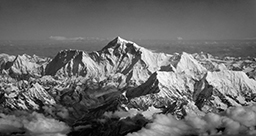
\includegraphics[width=0.9\textwidth]{./images/original.jpg}
      \caption{Original Image}
      \label{fig:original}
  \end{minipage}\hfill
  \begin{minipage}{0.45\textwidth}
      \centering
      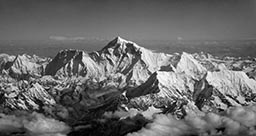
\includegraphics[width=0.9\textwidth]{./images/compressed.jpg}
      \caption{Compressed Image}
      \label{fig:compressed}
  \end{minipage}
\end{figure}

\section{Conclusion}
\label{sec: conclusion}

While the image was compressed by 40\% in file size, the compression is by not perfect, as evidenced by noticable artifacts around the edges of the mountain.
This makes sense when reviewing how JPEG compressing images.
Because the algorithm processes the data in 8x8 chunks and smooths out the data, the algorithm struggles with hard edges or areas where color changes sharply.
This is expecially noticable near the peak of the mountain where one can plainly see where each of the 8x8 chunks are.
However, while looking around at the rest of the image, nothing stands too far out of the ordinary.
When looking at the broad sides of the mountain or at the sky, other than a general loss in detail, the image looks outstanding for how much actual data is spared.

\section{Further Examples}
\label{sec: furtherexamples}

\begingroup
  \raggedright

  \nocite{*}
  \bibliographystyle{unsrtnat}
  \bibliography{bibliography}
\endgroup

\end{document}

